\section{CLI backend for Rainbow interpreter}

%\subsection{Promotion on CLI}
%
%Implementing promotion on top of CLI is not straightforward, as it needs to
%patch and modify the already generated code, and this is not possible on .NET.
%
%To solve, we do xxx and yyy etc. etc.
%

\subsection{Flexswitches}

As already explained, \dacom{I guess flexswitches will be introduced
  in the previous sect.} \emph{flexswitch} is one of the key
concepts allowing the JIT compiler generator to produce code which can
be incrementally specialized and compiled at run time.

A flexswitch is a special kind of switch which can be dynamically
extended with new cases; intuitively, its behavior can be described
well in terms of flow graphs. Indeed, a flexswitch can be considered 
as a special flow graph block where links to newly created blocks are
dynamically added whenever new cases are needed. 

\begin{figure}[h]
\begin{center}
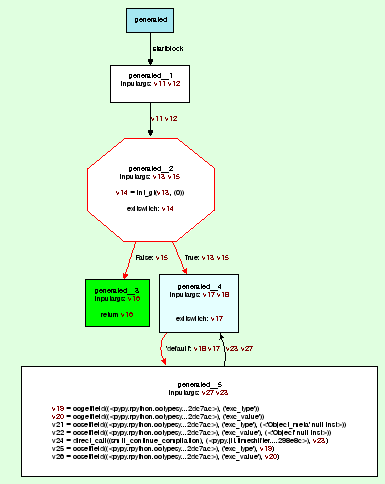
\includegraphics[height=5cm]{flexswitch1}
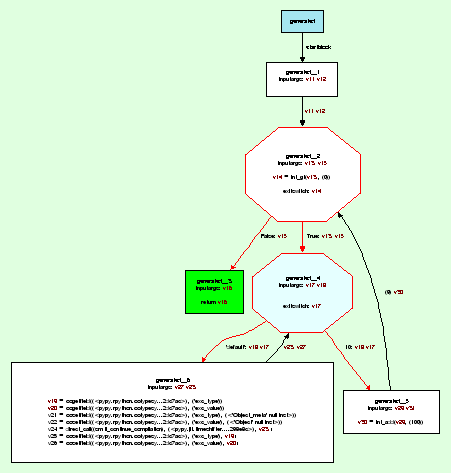
\includegraphics[height=5cm]{flexswitch2}
\caption{An example of a flexswitch evolution: in the picture on the
  right a new block has been dynamically added.}\label{flexswitch-fig}
\end{center}
\end{figure}

In the pictures of Figure~\ref{flexswitch-fig}, the cyan block
corresponds to a flexswitch; initially (picture on the left) 
only the block containing the code to restart the JIT compilation
is connected to the flexswitch; the picture on the right
shows the graph after the first case has been dynamically added to the flexswitch,
by linking the cyan block with a freshly created new block.


\subsection{Implementing flexswitches in CLI}

Implementing flexswitches for backends generating machine code is
not too complex: basically, a new jump has to be inserted in the
existing code to point to the newly generated code fragment.

Unfortunately, the CLI VM does not allow modification of code which
has been already loaded and linked, therefore the simplest approach
taken for low level architectures does not work for higher level 
virtual machines as those for .NET and Java.

Since in .NET methods are the basic units of compilation, a possible
solution consists in creating a new method 
any time a new case has to be added to a flexswitch.
\dacom{comment for Antonio: I am not sure this is the best solution. This cannot work for Java where classes are the basic
  units. Closures will be available only with Java Dolphin and I do
  not know how much efficient will be}
In this way, whereas flow graphs without flexswitches are translated
to a single method, the translation of flow graphs which can dynamically grow because of
flexswitches will be scattered over several methods.
Summarizing, the backend behaves in the following way:
\begin{itemize}
\item Each flow graph is translated in a collection of methods which
  can grow dynamically. \dacom{I propose primary/secondary instead of
    the overloaded terms main/child} Each collection contains at least one
  method, called \emph{primary}, which is the first to be created.
  All other methods, called \emph{secondary}, are added dynamically 
  whenever a new case is added to a flexswitch.

\item Each either primary or secondary method implements a certain
  number of blocks, all belonging to the same flow graph. Among these blocks
  there always exists an initial block whose input variables are
  parameters of the method; the input variables of all other blocks
  are local variables of the method.
\end{itemize} 

When  a new case is added to a flexswitch, new blocks are generated
and translated by the backend in a new single method pointed
by a delegate which is stored in the code implementing the flexswitch,
so that the method can be invoked later.

\subsubsection{Internal and external links}

A link is called \emph{internal} if it connects two blocks implemented
by the same method,
 \emph{external} otherwise.

Following an internal link is not difficult in IL bytecode: a jump to
the corresponding code fragment in the same method is emitted 
to execute the new block, whereas the appropriate local variables are
used for passing arguments.
Also following an external link whose target is the initial block of a
method is not difficult: the corresponding method has to be invoked
with the appropriate arguments.

What cannot be easily implemented in CLI is following an external link
whose target is not an initial block; consider, for instance, the
outgoing link of the block dynamically added in the right-hand side
picture of Figure~\ref{flexswitch-fig}. How it is possible to pass the
right arguments to the target block?

To solve this problem every method contains a special code, called
\emph{dispatcher}; whenever a method is invoked, its dispatcher is
executed first\footnote{The dispatcher should not be
confused with the initial block of a method.} to
determine which block has to be executed.
This is done by passing to the method a 32 bits number, called 
\emph{block id}, which uniquely identifies the next block of the graph to be executed.
The high word of a block id is the id of the method to which the block
belongs, whereas the low word is a progressive number univocally identifying
each block implemented by the method.

The picture in Figure~\ref{block-id-fig} shows a graph composed of three methods (for
simplicity, dispatchers are not shown); method ids are in red, whereas
block numbers are in black. 
The graph contains three external links; in particular, note the link
between blocks \texttt{0x00020001} and \texttt{0x00010001} which
connects two blocks implemented by different methods.
\begin{figure}[h]
\begin{center}
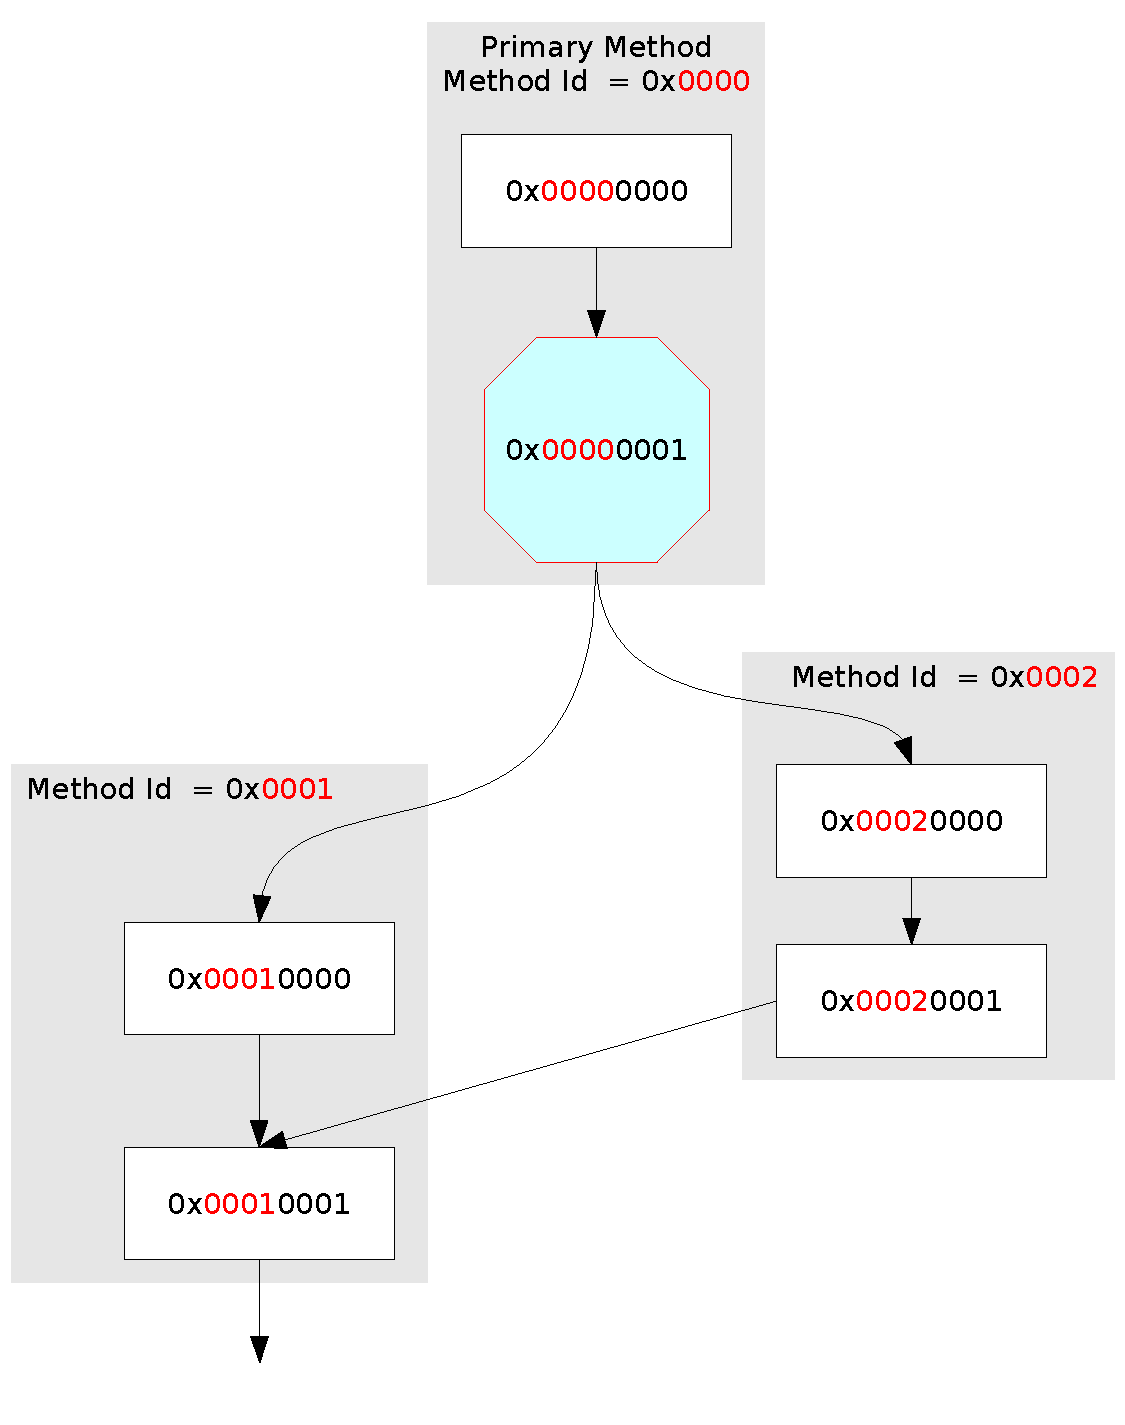
\includegraphics[height=6cm]{blockid}
\caption{Method and block ids.}\label{block-id-fig}
\end{center}
\end{figure}

For instance, the code\footnote{For simplicity we write C\# code instead of
the actual IL bytecode.} generated for the dispatcher of method \texttt{0x0002}
is similar to the following fragment: 
\begin{small}
\begin{lstlisting}[language={[Sharp]C}]
// dispatch block
int methodid = (blockid && 0xFFFF0000) >> 16; 
int blocknum = blockid && 0x0000FFFF;         
if (methodid != MY_METHOD_ID) {
  // jump_to_ext 
  ...
}
switch(blocknum) {
  case 0: goto block0;
  case 1: goto block1;
  default: throw new Exception("Invalid block id");
}
\end{lstlisting}
\end{small}
If the next block to be executed is implemented in the same method
({\small\lstinline{methodid == MY_METHOD_ID}}), then the appropriate
jump to the corresponding code is executed. Otherwise, the \lstinline{jump_to_ext}
part of the dispatcher has to be executed.
The code that actually jumps to an external block is contained in
the dispatcher of the primary method, whereas the
\lstinline{jump_to_ext} code of dispatchers of secondary methods
simply delegates the dispatcher of the primary method of the same
graph (see later).

The primary method is responsible for the bookkeeping of the secondary
methods which are added to the same graph dynamically. This can be 
simply implemented with an array mapping method id of secondary methods
to the corresponding delegate. Therefore, the primary methods contain
the following \lstinline{jump_to_ext} code (where
\lstinline{FlexSwitchCase} is the type of delegates for secondary methods):
\begin{small}
\begin{lstlisting}[language={[Sharp]C}] 
// jump_to_ext
FlexSwitchCase meth = method_map[methodid];
blockid = meth(blockid, ...); // execute the method
goto dispatch_block;
\end{lstlisting}
\end{small}
Each secondary method returns the block id of the next block to be
executed; therefore, after the secondary method has returned, the
dispatcher of the primary method will be executed again to jump
to the correct next block. 

To avoid mutual recursion and an undesired growth of the stack,
the \lstinline{jump_to_ext} code in dispatchers of secondary methods
just returns the block id of the next block; since the primary method
is always the first method of the graph which is called, the correct
jump will be eventually executed by the dispatcher of the primary method.

\commentout{
To implement the dispatch block we can exploit the switch opcode of the CLI; if the .NET JIT is smart enough, it can render it using an indirect jump; overall, jumping to a external block consists of an indirect function call (by invoking the delegate) plus an indirect jump (by executing the switch opcode); even if this is more costly than a simple direct jump, we will see in the next section that this not the main source of overhead when following a external link.

Obviously, the slow dispatching logic is needed only when we want to jump to a external block; if the target block happens to reside in the same method as the current one, we can directly jump to it, completely removing the overhead.

Moreover, the dispatch blocks are emitted only if needed, i.e. if the parent graph contains at least one flexswitch; graphs without flexswitches are rendered in the obvious way, by making one method per graph.

The slow bit: passing arguments

Jumping to the correct block is not enough to follow a link: as we said before, each link carries a set of arguments to be passed from the source to the target block. As usual, passing arguments across internal links is easy, as we can just use local variables to hold their values; on the other hand, external links make things more complex.

The only way to jump to a block is to invoke its containing method, so the first solution that comes to mind is to specify its input arguments as parameter of the method; however, each block has potentially a different number (and different types) of input arguments than every other block, so we need to think of something else.

An alternative solution could be to compute the union of the sets of input arguments of all the blocks in the method, and use this set as a signature for the method; this way, there would be enough space to specify the input arguments for every block we might want to jump to, each block ignoring the exceeding unused parameters.

Unfortunately, all the secondary methods must have the very same signature, as they are all called from the same calling site in the dispatch block of the main method. Since the union of the set of input arguments (and hence the computed signature) varies from method to method, this solution cannot work.

We might think to determine the signature by computing the union of input arguments of all blocks in the graph; this way, all the secondary methods would have the same signature. But as we said above, the graph grows new blocks at runtime, so we cannot determine in advance which set of input arguments we will need.

To solve the problem we need a way to pass a variable number of arguments without knowing in advance neither their number nor their types. Thus, we use an instance of this class:

public class InputArgs {
public int[] ints;
public float[] floats;
public object[] objs;
...
}

Since the fields are arrays, they can grow as needed to contain any number of arguments; arguments whose type is primitive are stored in the ints or floats array, depending on their type; arguments whose type is a reference type are stored in the objs array: it's up to each block to cast each argument back to the needed type.

This solution impose a huge overhead on both writing and reading arguments:

        * when writing, we need to make sure that the arrays are big enough to contains all the arguments we need; if not, we need to allocate a bigger array. Moreover, for each argument we store into the array the virtual machine performs a bound-check, even if we know the index will never be out of bounds (because we checked the size of the array in advance);
        * when reading, the same bound-check is performed for each argument read; moreover, for each value read from the objs array we need to insert a downcast.

To mitigate the performance drop, we avoid to allocate a new InputArgs object each time we do a external jump; instead, we preallocate one at the beginning of the main method, and reuse it all the time.

Our benchmarks show that passing arguments in arrays is about 10 times slower than passing them as real parameter of a method. Unfortunately, we couldn't come up with anything better.
Implement flexswitches

Now, we can exploit all this machinery to implement flexswitches, as this is our ultimate goal. As described above, the point is to be able to add new cases at runtime, each case represented as a delegate. Here is an excerpt of the C# class that implements a flexswitch that switches over an integer value:

public class IntLowLevelFlexSwitch:
{
public uint default_blockid = 0xFFFFFFFF;
public int numcases = 0;
public int[] values = new int[4];
public FlexSwitchCase[] cases = new FlexSwitchCase[4];

public void add_case(int value, FlexSwitchCase c)
{
...
}

public uint execute(int value, InputArgs args)
{
for(int i=0; i<numcases; i++)
if (values[i] == value) {
 return cases[i](0, args);
}
return default_blockid;
}
}

For each case, we store both the triggering value and the corresponding delegate; the add_case method takes care to append value and c to the values and cases arrays, respectively (and resize them if necessary). The interesting bit is the execute method: it takes a value and a set of input arguments to be passed across the link and jumps to the right block by performing a linear search in the values array.

As shown by previous sections, the first argument of a FlexSwitchCase is the block id to jump to; since when we go through a flexswitch we always want to jump to the first block of the method, we pass the special value 0 as a block id, which precisely means jump to the first block. This little optimization let us not to have to explicitly store the block id for the first block of all the cases.

The value returned by execute is the next block id to jump to; if the value is not found in the values array, we return the default_blockid, whose value has been set before by the JIT compiler; default_blockid usually points to a block containing code to restart the JIT compiler again; when the JIT compiler restarts, it emits more code for the missing case, then calls add_case on the flexswitch; from now on, the new blocks are wired into the existing graph, and we finally managed to implement growable graphs.
Performances

As we saw, implementing growable graphs for CLI is a pain, as the virtual machine offers very little support, so we need an incredible amount of workarounds. Moreover, the code generated is much worse than what an assembly backend could produce, and the cost of following a external link is very high compared to internal links.

However, our first blog post showed that we still get very good performances; how is it possible?

As usual in computer science, most of the time of a running program in spent in a tiny fraction of the code; our benchmark is no exception, and the vast majority of the time is spent in the inner loop that multiplies numbers; the graph is built in such a way that all the blocks that are part of the inner loop reside in the same method, so that all links inside are internal (and fast).

Flexswitches and external links play a key role to select the right specialized implementation of the inner loop, but once it is selected they are not executed anymore until we have finished the computation.

It is still unclear how things will look like when we will compile the full Python language instead of a toy one; depending on the code, it could be possible to have external links inside the inner loop, thus making performance much worse.
Alternative implementations

Before implementing the solution described here, we carefully studied a lot of possible alternatives, but all of them either didn't work because of a limitation of the virtual machine or they could work but with terrible performances.

In particular, in theory it is possible to implement external links using tail calls, by putting each block in its own method and doing a tail call instead of a jump; this would also solve the problem of how to pass arguments, as each method could have its own signature matching the input args of the block. I would like to explain this solution in a more detailed way as I think it's really elegant and nice, but since this post is already too long, I'll stop here :-).

In theory, if the .NET JIT were smart enough it could inline and optimize away the tail calls (or at least many of those) and give us very efficient code. However, one benchmark I wrote shows that tail calls are up to 10 times slower (!!!) than normal calls, thus making impractical to use them for our purposes.
Conclusion

Despite the complexity of the implementation, our result are extremely good; the speedup we got is impressive, and it proves that PyPy's approach to JIT compiler can work well also on top of object oriented virtual machines like .NET or the JVM.

Generating bytecode for those machine at runtime is not a new idea; Jython, IronPython, JRuby and other languages have been doing this for years. However, Jython and IronPython do only a simple "static" translation, which doesn't take advantage of the informations gathered at runtime to generate better, faster and specialized code. Recently, JRuby grew a new strategy to JIT-compile only hotspots, taking advantage of some informations gathered while interpreting the code; this is still a "one-shot" compilation, where the compiled code does not change over time.

To my knowledge, PyPy brings the first example of a language which implements a truly JIT compiler on top of the underlying JIT compiler of the virtual machine, emitting bytecode that changes and adapts over the time. If someone knows other languages doing that, I would really like to know more.

Being so innovative, the problem of this approach is that the current virtual machines are not designed to support it in a native way, and this forces us to put a lot of workarounds that slow down the generated code. The hope is that in the future the virtual machines will grow features that help us to generate such kind of code. The experimental Da Vinci VM seems to go in the right direction, so it is possible that in the future I will try to write a JIT backend for it.

At the moment, the CLI JIT backend is almost complete, and all the hardest problems seems to be solved; the next step is to fix all the remaining bugs and implement some minor feature that it's still missing, then try to apply it to the full Python language and see what is the outcome.
}

% LocalWords:  flexswitches backend flexswitch methodid blockid xFFFF blocknum
% LocalWords:  FFFF goto FlexSwitchCase meth
